\documentclass[12pt, a4paper]{article}
\usepackage{amsmath}
\usepackage{amsfonts}
\usepackage{amsthm}
\usepackage{mathtools}
\newtheorem{theorem}{Theorem}[section]
\newtheorem{definition}{Definition}[section]
\numberwithin{equation}{section}
\usepackage{pgfplots}
\pgfplotsset{width=10cm,compat=1.9}
\graphicspath{ {img/} }
\DeclareGraphicsExtensions{.png}
\DeclareGraphicsExtensions{.jpg}

\title{Single value decomposition and pseudo-inverses}
\author{Kristian Wichmann}

\begin{document}
\maketitle

\section{Gramian matrices}
Given a set of vectors $a_1, a_2,\ldots, a_n\in\mathbb{R}^m$, the Gramian matrix is the traditionally matrix of inner products $\langle a_i,a_j\rangle$. If these vectors are collected into a $m\times  n$ matrix $A$, this matrix can be expressed as $A^t A$. Here, we will use the term for any matrix in this form. By starting out with the transpose instead, this means that $AA^t$ is also a Gramian, with dual results.

\begin{theorem}
\label{gramian_basic}
If $A\in\mathbb{R}^{m\times n}$, then $A^t A$ is symmetric and positive semi-definite. Iff $A$ has rank $m$, $A^t A$ is positive definite.
\end{theorem}
\begin{proof}
$(A^t A)^t=A^t(A^t)^t=A^t A$ shows symmetry. positive semi-definiteness, let $x\in\mathbb{R}^n$. Then:
\begin{equation}
x^t A^t Ax=\langle Ax,Ax\rangle=||Ax||^2
\end{equation}
As a norm, this is greater than or equal to zero. Hence $A^t A$ is positive semi-definite. If $A$ has rank $m$ the map $x\mapsto Ax$ has a trivial kernel by the rank-kernel theorem. Which means only the zero vector is mapped to zero, and hence $A^t A$ is positive definite. If the rank is less than $m$, the kernel is non-trivial and positive definiteness cannot be true.
\end{proof}

\section{The rank-nullity theorem}

\subsection{For $A$ and $A^t$}
According to the rank-nullity theorem, for a matrix $A\in\mathbb{R}^{m\times n}$, the sum of the rank and nullity is $n$. So, if the rank of $A$ is $r$, then $\textrm{null}A=n-r$. Applying the theorem to $A^t$, which also has rank $r$, we get $\textrm{null}A=m-r$.

The image of $A$ is also called the \textit{column space} of $A$, denoted $C(A)$. The image of $A^t$ is also called the \textit{row space} of $A$, $C(A^t)$. The null space of $A^t$ is often called the \textit{left null space}.

\begin{figure}
\centering
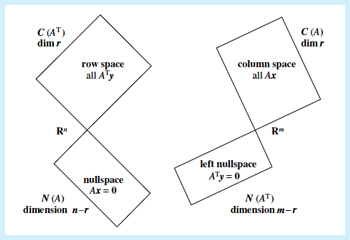
\includegraphics[width=\textwidth]{row_column_null}
\caption{Visualization of dimensionality for the rank-nullity theorem}
\label{fig:rank-nullity}
\end{figure}

These relationships are visualized in figure \ref{fig:rank-nullity}.

\section{Single value decomposition}
Let $A\in\mathbb{R}^{m\times n}$. Since $A^t A$ is symmetric, it is diagonalizable. So there is an orthogonal $n\times n$ matrix $O$ such that $A^t A=ODO^t$, where $D$ is a diagonal matrix of eigenvalues. 

\section{Orthogonal projection}
Let $U$ be a subspace of $\mathbb{R}^n$ spanned by the linearly independent set of vectors $a_1, a_2,\ldots, a_m$. Given a $x\in\mathbb{R}^n$, we wish to find a vector $u$ in $U$, such that $e=x-u$ is orthogonal to $U$. That means it should be orthogonal to all $a_i$'s:
\begin{equation}
\forall i:\ a_i^t(x-u)=0
\end{equation}
This can be expressed in matrix form by collecting all the $a_i$'s into a $n\times m$ matrix $A$:
\begin{equation}
A=
\begin{pmatrix}
|	&	|	&	\cdots	&	|\\
a_1	&	a_2	&	\cdots	&	a_m\\
|	&	|	&	\cdots	&	|
\end{pmatrix}
\end{equation}
Then we may write:
\begin{equation}
A^t(x-u)=0
\end{equation}
Since $u\in U$, it can be written as a linear combination of $a_i$'s, so $u=A\beta$. We want to solve for the coefficient vector $\beta$:
\begin{equation}
A^t(x-A\beta)=0\Leftrightarrow A^t x=A^t A\beta
\end{equation}
Since the $a_i$'s are linearly independent, $A^t A$ is invertible, so: 
\begin{equation}
\beta=(A^t A)^{-1}A^t x
\end{equation}
The actual vector is then $A\beta=A(A^t A)^{-1}A^t x$. Which means that the projection operator $p_U:\mathbb{R}^n\rightarrow U$ is linear with the corresponding matrix being $P_U=A(A^t A)^{-1}A^t$.

\begin{theorem}
\label{projection_characterization}
The matrix $P_U$ is symmetric and idempotent.
\end{theorem}
\begin{proof}
Both follow directly from the formula $P_U=A(A^t A)^{-1}A^t$:
\begin{itemize}
\item Symmetry: $P_U^t=\left(A(A^t A)^{-1}A^t\right)^t=A\left[(A^t A)^{-1}\right]^t A^t$. But since the transpose of an inverse is the inverse of a transpose, and $A^t A$ is symmetric by theorem \ref{gramian_basic} we have $\left[(A^t A)^{-1}\right]^t=\left[(A^t A)^t\right]^{-1}=(A^t A)^{-1}$. Hence $P_U^t=A(A^t A)^{-1}A^t=P_U$.
\item Idempotency: $P_U^2=\left(A(A^t A)^{-1}A^t\right)^2=A(A^t A)^{-1}A^t A(A^t A)^{-1}A^t=A(A^t A)^{-1}A^t=P_U$.
\end{itemize}
\end{proof}

\section{Generalized inverses}
For an invertible matrix $A$, it's obviously true that:
\begin{equation}
AA^{-1} A=A
\end{equation}
If $A$ is not invertible, we may still define a \textit{generalized inverse} $A^g$ as a matrix that satisfies the same equation:
\begin{equation}
\label{generalized_inverse}
AA^g A=A
\end{equation}
If $A^g$ further satisfies:
\begin{equation}
\label{reflexive_generalized_inverse}
A^g AA^g=A^g,
\end{equation}
it is called a \textit{reflexive generalized inverse}.

\subsection{Left and right inverses}
If $A\in\mathbb{R}^{m\times n}$ has rank $n$, then the null space is trivial, and hence the corresponding linear transformation is injective. This means that the equation $Ax=b$ may or may not have a solution, but if it exists, it's unique. The matrix $A^tA$ has rank $n$ as well, and hence is invertible. This can be used to construct a left inverse:
\begin{equation}
A^{-1}_L=(A^t A)^{-1}A^t,\qquad A^{-1}_L A=(A^t A)^{-1}A^t A=I_n
\end{equation}

Similarly, if $A\in\mathbb{R}^{m\times n}$ has rank $m$, then the image space is all of $\mathbb{R}^m$, and hence the corresponding linear transformation is surjective. This means that the equation $Ax=b$ always has a solution, and it may have infinitely many. The matrix $AA^t$ has rank $m$ as well, and hence is invertible. Analogously, we can use this to construct a right inverse:
\begin{equation}
A^{-1}_R=A^t(AA^t)^{-1},\qquad AA^{-1}_R=AA^t(AA^t)^{-1}=I_m
\end{equation}

Both of of these inverses (when they exist) satisfies equation \ref{generalized_inverse}. They also satisfy \ref{reflexive_generalized_inverse}. For instance:
\begin{equation}
A^{-1}_L AA^{-1}_L=(A^t A)^{-1}A^t A(A^t A)^{-1}A^t=(A^t A)^{-1}A^t=A^{-1}_L
\end{equation}
So both are reflexive, generalized inverses.

\section{The Moore-Penrose pseudoinverse}
The \textit{Moore-Penrose pseudoinverse} or simply the pseudoinverse of a real matrix $A$ is the reflexive, generalized inverse $A^+$ which also satisfies:
\begin{equation}
\label{moore-penrose}
(AA^+)^t=AA^+,\qquad(A^+ A)^t=A^+ A
\end{equation}
In other words, for which $AA^+$ and $A^+ A$ are symmetrical.

\subsection{Uniqueness}
If such a pseudoinverse exists, it is unique (hence our use of definite article above). To show this, let $B_1$ and $B_2$ be pseudoinverses of $A$. Then:
\begin{align}
AB_1=(AB_1)^t=B_1^t A^t=B_1^t(AB_2 A)^t=B_1^t A^t B_2^t A^t=&\\
(AB_1)^t(AB_2)^t=AB_1 AB_2=&AB_2
\end{align}
Similarly:
\begin{align}
B_1A=(B_1A)^t=A^t B_1^t=(AB_2 A)^t B_1^t=A^t B_2^t A^t B_1^t=&\\
(B_2 A)^t(B_1 A)^t=B_2 A B_1 A=&B_2 A
\end{align}
But then:
\begin{equation}
B_1=B_1 AB_1=B_2 AB_1=B_2 AB_2=B_2
\end{equation}

\end{document}